\documentclass[12pt]{article}
\usepackage[utf8]{inputenc}
\usepackage{graphicx}
\usepackage{subcaption}
\usepackage{amsmath}
\usepackage{fancyhdr}
\usepackage{geometry}
\usepackage{dirtytalk}
\usepackage[english]{babel}
\usepackage{csquotes}
\usepackage{hyperref}
\usepackage{xcolor}
\usepackage{booktabs}
\usepackage{longtable}
\usepackage{array}
\usepackage[T1]{fontenc}
\usepackage{float}

\linespread{1.25}
\setlength{\parindent}{0.8cm}
\setlength{\parskip}{0em}
\renewcommand{\headrulewidth}{0pt}
\geometry{a4paper, portrait, margin=1in}
\setlength{\headheight}{14.49998pt}
\graphicspath{{./}{../}}

% ============================================================================
\begin{document}

% ---------------------------------------------------------------------------
% TITLE PAGE
% ---------------------------------------------------------------------------
\begin{titlepage}
  \begin{center}
    \textsc{\large Ministry of Education of Republic of Moldova}\\[0.5cm]
    \textsc{\large Technical University of Moldova}\\[0.5cm]
    \textsc{\large Faculty of Computers, Informatics and Microelectronics}\\[0.5cm]
    \textsc{\large Software Engineering Department}\\[1.2cm]

    \vspace{20mm}
    \textsc{\Large Embedded Systems}\\[0.5cm]
    \textsc{\large Laboratory Work \#5}\\[0.5cm]

    \newcommand{\HRule}{\rule{\linewidth}{0.5mm}}
    \vspace{8mm}
    \HRule\\[0.4cm]
    {\LARGE \bfseries Dual-Sensor Temperature Monitor\\[0.2cm]
    \large Signal Acquisition, Binary Threshold Conditioning, and LCD Reporting\\[0.3cm]}
    \HRule\\[1.5cm]

    \begin{minipage}[t]{0.45\textwidth}
      \begin{flushleft}\large
        \emph{Author:}\\
        Sava \textsc{Luchian}\\
        std. gr. FAF-233
      \end{flushleft}
    \end{minipage}
    ~
    \begin{minipage}[t]{0.45\textwidth}
      \begin{flushright}\large
        \emph{Verified:}\\
        Alexei \textsc{Martiniuc}\\
      \end{flushright}
    \end{minipage}\\[2.5cm]

    \large Chisinau 2026
    \vfill
  \end{center}
\end{titlepage}

\setcounter{page}{2}
\pagestyle{fancy}
\fancyhf{}
\rhead{\thepage}
\lhead{FAF-233 Sava Luchian; Laboratory Work No.\ 5}

% ---------------------------------------------------------------------------
% TECHNICAL TASK
% ---------------------------------------------------------------------------
\section*{Technical Task}

\subsection*{Purpose of the Laboratory}
\hspace{0.8cm} Familiarise students with sensor signal acquisition and conditioning techniques on embedded microcontrollers by implementing a dual-sensor temperature monitoring application that periodically reads two sensors (one analogue NTC thermistor, one digital DHT22), applies a binary threshold filter with hysteresis and persistence confirmation to each channel, drives visual and audible alerts, and reports all intermediate processing states via STDIO (\texttt{printf}) and a 16$\times$2 LCD display.

\subsection*{Objectives}
\begin{enumerate}
    \item Read raw data from an analogue sensor (NTC thermistor via ADC) and a digital sensor (DHT22 via 1-Wire) at a configurable acquisition rate (40\,ms).
    \item Read a potentiometer on A1 and map it to a configurable temperature setpoint in the range 20--35\,°C (bonus functionality).
    \item Apply a multi-stage signal conditioning pipeline: voltage conversion, B-model resistance-to-temperature calculation, binary threshold detection with hysteresis and persistence debouncing.
    \item Display processed sensor values, conditioning state, and alert status on a 16$\times$2 LCD and via STDIO \texttt{printf} at a 500\,ms reporting rate.
    \item Drive a green/red LED pair and a passive buzzer to provide immediate alert feedback.
    \item Demonstrate clean modular software architecture separating sensors, signal conditioning, peripherals, I/O, and application logic.
\end{enumerate}

\subsection*{Individual Task}
\hspace{0.8cm} Design and implement on an \textbf{Arduino Uno (ATmega328P)} a bare-metal (non-FreeRTOS) dual-sensor monitoring application structured as follows:

\begin{itemize}
    \item \textbf{NTC Sensor} -- Analogue thermistor on pin A0; read ADC raw, convert to voltage, compute resistance via voltage-divider model, compute temperature with the B-parameter (Steinhart--Hart) equation.
    \item \textbf{DHT22 Sensor} -- Digital temperature/humidity sensor on D8; read via Adafruit DHT library; cache last valid value when the sensor returns NaN within the 2\,s recharge window.
    \item \textbf{Potentiometer (Bonus)} -- Analogue input on A1; mapped to setpoint interval 20--35\,°C. Dynamic thresholds are computed as: \texttt{high=setpoint+1.0}, \texttt{low=setpoint-1.0}.
    \item \textbf{Binary Threshold Filter} -- One instance per sensor; hysteresis thresholds are updated at runtime from the potentiometer setpoint; persistence confirmation: 2 consecutive samples before state change ($\leq$\,80\,ms confirmation at 40\,ms acquisition); prevents oscillation near the threshold.
    \item \textbf{Alert Output} -- \textbf{Red LED} + \textbf{Buzzer ON} when either sensor triggers \texttt{stableHigh}; \textbf{Green LED} otherwise.
    \item \textbf{Reporting} -- Every 500\,ms: \texttt{printf} full diagnostic dump (raw ADC, voltage, temperature, candidateHigh, stableHigh, pending counter) for both channels plus potentiometer raw/setpoint and thresholds; LCD shows \texttt{N:xx.x D:xx.x} and \texttt{TH:high/low}.
\end{itemize}

% ---------------------------------------------------------------------------
% SECTION 1 — DOMAIN ANALYSIS
% ---------------------------------------------------------------------------
\section{Domain Analysis}

\subsection{Technological Context and Application Domain}
\hspace{0.8cm} Temperature monitoring is one of the most common applications in embedded systems. From industrial process control to consumer IoT devices, reliable acquisition and conditioning of thermal data underpins safe and correct system operation. This laboratory targets the full signal processing chain from physical transducer to user-visible output:

\begin{itemize}
    \item \textbf{Analogue sensing}: An NTC (Negative Temperature Coefficient) thermistor changes resistance non-linearly with temperature. The MCU's 10-bit ADC converts the divider voltage to a digital value; software then applies the B-parameter (Steinhart--Hart) model to recover temperature in °C.
    \item \textbf{Digital sensing}: The DHT22 (AM2302) encodes temperature and humidity as a single-wire serial bitstream. The Adafruit DHT library handles the protocol timing; the application layer deals only with floating-point temperature values and error recovery.
    \item \textbf{Binary threshold conditioning}: Raw temperature readings are inherently noisy near a decision boundary. A hysteresis band (high/low threshold pair) combined with a persistence counter prevents repeated alert toggling when the temperature hovers around the set-point -- a standard industrial technique also known as ``bang-bang with hysteresis.''
    \item \textbf{Multi-rate loop}: Acquisition runs at 40\,ms (sensor-dictated minimum); LCD/STDIO reporting runs at 500\,ms to avoid flooding the display. This decoupling of acquisition from reporting is the canonical embedded real-time pattern.
\end{itemize}

\subsection{Hardware Components and Justification}

\begin{table}[H]
\centering
\begin{tabular}{p{4.2cm} p{1.8cm} p{7cm}}
\toprule
\textbf{Component} & \textbf{Qty} & \textbf{Role in the application} \\
\midrule
Arduino Uno (ATmega328P) & 1 & Main MCU; 16\,MHz, 2\,KB SRAM, 32\,KB Flash. 10-bit ADC for NTC; GPIO for DHT22 and LCD. \\
NTC Thermistor (10\,k$\Omega$ @ 25\,°C, B=3950\,K) & 1 & Analogue temperature sensor; connected with a 10\,k$\Omega$ fixed resistor in voltage-divider configuration to A0. \\
Potentiometer (10\,k$\Omega$) & 1 & User-controlled setpoint selector on A1. Mapped in software to 20--35\,°C and used to compute dynamic threshold pair. \\
DHT22 (AM2302) & 1 & Digital temperature + humidity sensor; 1-Wire protocol on D8. Accuracy $\pm$0.5\,°C. \\
16$\times$2 LCD (LiquidCrystal, 4-bit) & 1 & Real-time display of NTC temperature, DHT22 temperature, and alert state. \\
Green LED + 220\,$\Omega$ & 1 & Normal-operation indicator (no alert). \\
Red LED + 220\,$\Omega$ & 1 & Alert indicator (either sensor above threshold). \\
Passive buzzer & 1 & Audible alert at 1\,kHz when alert is active. \\
10\,k$\Omega$ resistor (fixed divider) & 1 & Voltage-divider partner for NTC. \\
Breadboard + jumper wires & -- & Prototyping interconnection. \\
USB cable & 1 & 5\,V power and serial communication (115\,200 baud). \\
\bottomrule
\end{tabular}
\caption{Hardware components used in Lab 5}
\label{tab:hardware}
\end{table}

\subsection{Software Components and Technologies}

\begin{itemize}
    \item \textbf{PlatformIO + VS Code}: Single \texttt{uno} environment. Arduino framework, no RTOS.
    \item \textbf{Arduino Framework (avr-arduino)}: GPIO, ADC (\texttt{analogRead}), \texttt{millis()}, \texttt{tone}/\texttt{noTone}, \texttt{LiquidCrystal} library.
    \item \textbf{Adafruit DHT sensor library 1.4.6}: Handles the DHT22 single-wire protocol; internally caches readings for 2\,s.
    \item \textbf{arduino-libraries/LiquidCrystal 1.0.7}: 4-bit parallel interface to HD44780-compatible 16$\times$2 LCD.
    \item \textbf{AVR-libc stdio}: \texttt{fdev\_setup\_stream} + \texttt{printf} redirected to Serial UART via \texttt{StdioBridge}. \texttt{dtostrf()} used for float formatting (AVR has no \texttt{\%f} in default \texttt{printf}).
    \item \textbf{Wokwi Simulator}: Circuit and firmware simulation in VS Code for functional testing.
\end{itemize}

\subsection{Analysis of Existing Solutions}
\hspace{0.8cm} Several design decisions were made over alternative approaches:

\begin{itemize}
    \item \textbf{Bare-metal vs.\ FreeRTOS}: Because the acquisition pipeline is simple (two sensors, one conditioning step, one report) and latency requirements are soft ($\leq$\,100\,ms), a cooperative bare-metal loop using \texttt{millis()} timestamps is sufficient and avoids the FreeRTOS RAM overhead ($\approx$\,400\,B for task stacks + TCBs) on the 2\,KB ATmega328P.
    \item \textbf{NTC B-parameter vs.\ lookup table}: The B-parameter (Steinhart--Hart two-point) model requires only two ROM constants and one \texttt{log()} call. A LUT requires 20--30 entries plus interpolation code. For the target 0--50\,°C range the B-model error is $<$\,0.5\,°C -- acceptable for this application.
    \item \textbf{Hysteresis + persistence vs.\ simple threshold}: A single threshold produces rapid oscillation when the temperature fluctuates near the set-point. The hysteresis band around a dynamic setpoint (controlled by potentiometer) prevents state changes in the neutral zone; the 2-sample persistence filter additionally suppresses single-sample noise spikes.
    \item \textbf{DHT22 vs.\ DHT11}: DHT22 provides $\pm$0.5\,°C accuracy vs.\ $\pm$2\,°C for DHT11, and covers a wider range. The 2\,s minimum read interval is handled transparently by the Adafruit library.
\end{itemize}

\subsection{Real-World Applications}
\hspace{0.8cm} The design patterns in this laboratory appear directly in commercial embedded products:

\begin{itemize}
    \item \textbf{HVAC controllers}: Hysteresis-based thermostat logic (identical to \texttt{BinaryThresholdFilter}) prevents compressor short-cycling by requiring temperature to fall below the low threshold before the cooling call is removed.
    \item \textbf{Industrial process monitors}: Dual-sensor redundancy (NTC + DHT22) is standard practice for critical temperature monitoring -- if one sensor fails, the other provides fallback.
    \item \textbf{Cold-chain logistics}: NTC thermistor arrays with B-model conversion are standard in IoT temperature loggers for pharmaceutical and food transport.
    \item \textbf{Server room monitoring}: LCD + STDIO reporting mirrors rack monitoring panels that show live sensor data and alarm state simultaneously on a local display and a remote serial/network interface.
    \item \textbf{Fire alarm panels}: Persistence confirmation (requiring stable over-threshold readings for N consecutive samples) is mandatory in EN 54-compliant fire detectors to prevent false alarms from transient heat sources.
\end{itemize}

% ---------------------------------------------------------------------------
% SECTION 2 — CONCEPTUALISATION AND DESIGN
% ---------------------------------------------------------------------------
\section{Conceptualisation and Design}

\subsection{Technical Requirements}

\begin{longtable}{p{1.5cm} p{2.5cm} p{7.5cm} p{1.5cm}}
\toprule
\textbf{ID} & \textbf{Category} & \textbf{Requirement} & \textbf{Type} \\
\midrule
\endfirsthead
R-F-01 & NTC & System shall read NTC ADC raw value at every acquisition cycle. & Func. \\
R-F-02 & NTC & System shall convert ADC raw to voltage, resistance, and temperature (B-model). & Func. \\
R-F-03 & DHT22 & System shall read DHT22 temperature at every acquisition cycle; cache last valid value on NaN. & Func. \\
R-F-04 & Conditioning & System shall apply hysteresis threshold per sensor with dynamic pair \texttt{high=setpoint+1.0}, \texttt{low=setpoint-1.0}. & Func. \\
R-F-05 & Conditioning & System shall require 2 consecutive confirming samples before changing stable state. & Func. \\
R-F-05a & Potentiometer & System shall read potentiometer (A1) and map ADC 0..1023 to setpoint 20..35\,°C. & Func. \\
R-F-06 & Alert & Red LED shall illuminate when either sensor \texttt{stableHigh} is true. & Func. \\
R-F-07 & Alert & Green LED shall illuminate when no sensor \texttt{stableHigh} is active. & Func. \\
R-F-08 & Alert & Buzzer shall sound at 1\,kHz when alert is active; shall be silent otherwise. & Func. \\
R-F-09 & LCD & LCD row 0 shall show NTC temperature and DHT22 temperature (or ``n/a'' if invalid). & Func. \\
R-F-10 & LCD & LCD row 1 shall show live threshold pair in format \texttt{TH:high/low} and alert marker. & Func. \\
R-F-11 & STDIO & Every 500\,ms: \texttt{printf} NTC raw, voltage, temperature, conditioner state, DHT22 temperature, conditioner state, and system alert. & Func. \\
R-F-12 & STDIO & System shall print configuration banner on startup via \texttt{printf}. & Func. \\
R-NF-01 & Latency & Alert state shall reflect sensor readings within 100\,ms of threshold crossing. & Non-func. \\
R-NF-02 & Memory & Firmware shall fit within 32\,KB Flash and 2\,KB SRAM. & Non-func. \\
R-NF-03 & Modularity & Application shall be structured in dedicated modules: config, sensors, signal, peripherals, io, app. & Non-func. \\
R-NF-04 & STDIO & All text output shall use \texttt{printf} via a \texttt{stdout} $\rightarrow$ Serial bridge. & Non-func. \\
R-NF-05 & Robustness & System shall not crash when DHT22 returns NaN; cached value shall be used. & Non-func. \\
\bottomrule
\caption{Technical requirements for Lab 5}
\label{tab:requirements}
\end{longtable}

\subsection{Architectural Design}

\subsubsection{System Structural Architecture}

The application follows a five-layer hardware--software boundary:

\begin{figure}[H]
\centering
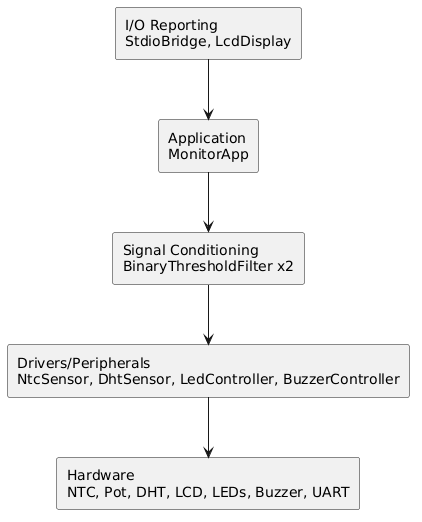
\includegraphics[width=0.88\textwidth]{layers.png}
\caption{Layered software architecture -- Lab 5}
\label{fig:layers}
\end{figure}

\subsubsection{HW/SW Interface and Component Interaction}

\begin{figure}[H]
\centering
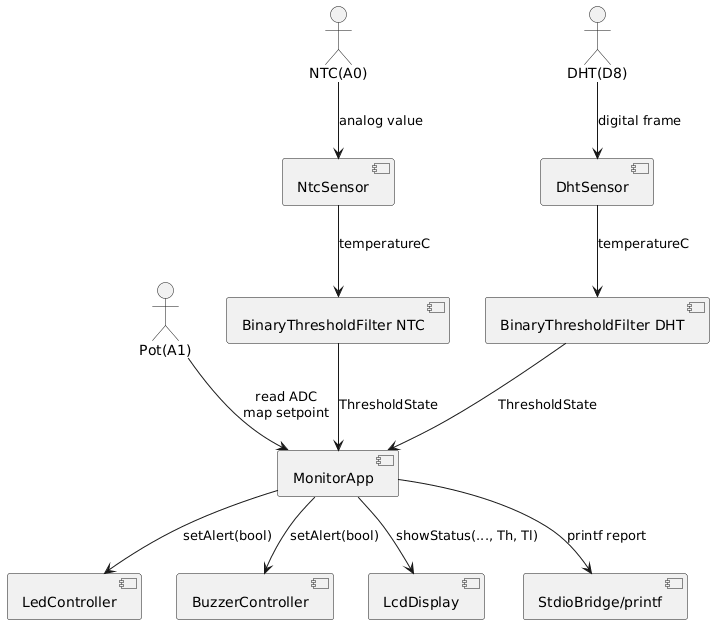
\includegraphics[width=0.88\textwidth]{interaction.png}
\caption{Component interaction diagram -- Lab 5}
\label{fig:interaction}
\end{figure}

\subsubsection{Signal Conditioning Pipeline Design}

The NTC signal conditioning pipeline (plus dynamic threshold update from potentiometer) consists of sequential stages:

\begin{figure}[H]
\centering
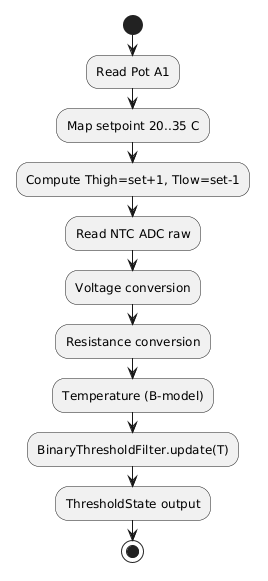
\includegraphics[width=0.88\textwidth]{ntc_pipeline.png}
\caption{NTC signal conditioning pipeline}
\label{fig:ntc-pipeline}
\end{figure}

\subsubsection{BinaryThresholdFilter State Machine}

The filter implements a two-state machine with hysteresis and persistence confirmation:

\begin{figure}[H]
\centering
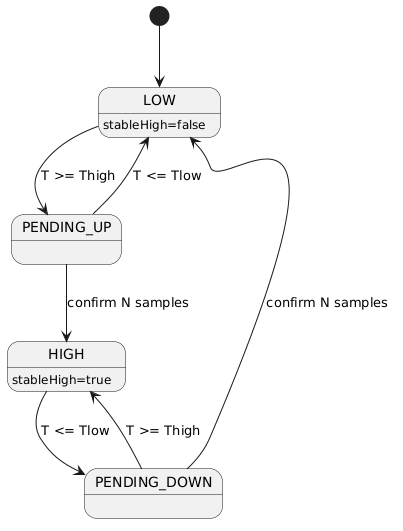
\includegraphics[width=0.88\textwidth]{threshold_fsm.png}
\caption{BinaryThresholdFilter state machine with hysteresis and persistence}
\label{fig:threshold-fsm}
\end{figure}

\subsubsection{Main Loop Timing Design}

The application uses a cooperative \texttt{millis()}-based multi-rate loop in \texttt{MonitorApp::tick()}:

\begin{table}[H]
\centering
\begin{tabular}{llll}
\toprule
\textbf{Activity} & \textbf{Period} & \textbf{Trigger} & \textbf{Handler} \\
\midrule
Sensor acquisition + conditioning & 40\,ms & \texttt{millis()} elapsed & \texttt{runAcquisitionAndConditioning()} \\
STDIO + LCD reporting & 500\,ms & \texttt{millis()} elapsed & \texttt{runReport()} \\
\bottomrule
\end{tabular}
\caption{Multi-rate loop timing}
\label{tab:timing}
\end{table}

Both rates share the same \texttt{loop()} call, with independent \texttt{lastAcquisitionMs} and \texttt{lastReportMs} timestamps. This is equivalent to a cooperative scheduler with two periodic tasks.

\subsubsection{STDIO Bridge Design}

On AVR, \texttt{printf} writes to \texttt{stdout} which is not connected to the serial port by default. \texttt{StdioBridge::begin()} registers a \texttt{serial\_putchar} function via \texttt{fdev\_setup\_stream}, redirecting each character to \texttt{Serial.write()} with automatic \texttt{\textbackslash{}n} $\rightarrow$ \texttt{\textbackslash{}r\textbackslash{}n} conversion. Because AVR \texttt{printf} has no \texttt{\%f} support in the default vfprintf variant, all floating-point values are pre-formatted with \texttt{dtostrf()} into local char buffers and printed as \texttt{\%s}.

\subsection{Behavioural Modelling}

\subsubsection{MonitorApp tick() Flowchart}

\begin{figure}[H]
\centering
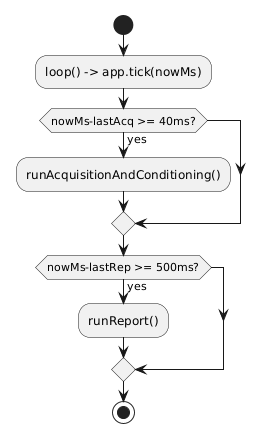
\includegraphics[width=0.88\textwidth]{tick_flow.png}
\caption{MonitorApp tick() flowchart -- two-rate cooperative loop}
\label{fig:tick-flow}
\end{figure}

\subsubsection{Acquisition and Conditioning Flowchart}

\begin{figure}[H]
\centering
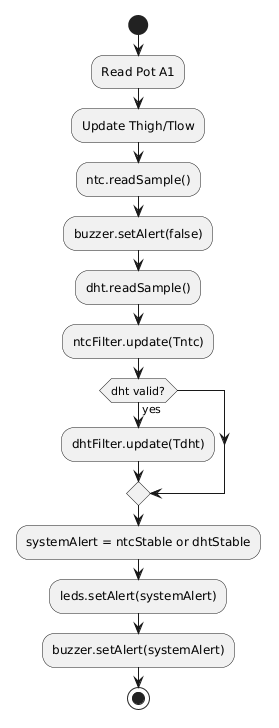
\includegraphics[width=0.88\textwidth]{acq_flow.png}
\caption{runAcquisitionAndConditioning() flowchart}
\label{fig:acq-flow}
\end{figure}

\subsubsection{Sequence Diagram -- Full Acquisition Cycle}

\begin{figure}[H]
\centering
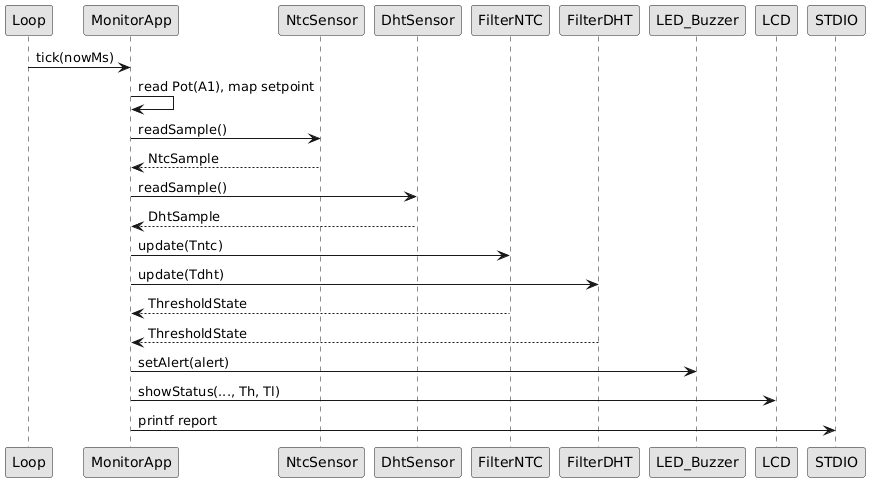
\includegraphics[width=0.92\textwidth]{sequence_cycle.png}
\caption{Sequence diagram -- full acquisition and reporting cycle}
\label{fig:sequence}
\end{figure}

\subsubsection{System State Machine}

\begin{figure}[H]
\centering
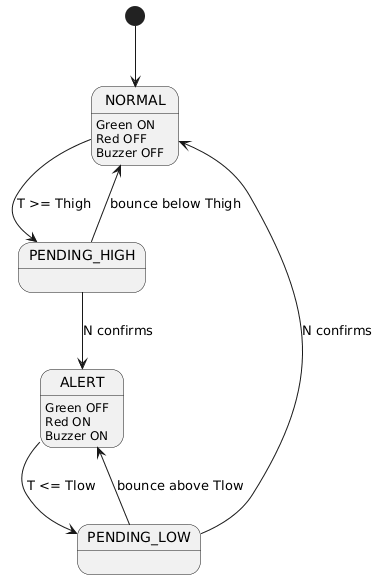
\includegraphics[width=0.88\textwidth]{system_fsm.png}
\caption{System-level state machine -- alert logic with pending state}
\label{fig:system-fsm}
\end{figure}

\subsection{Test Scenarios and Validation Criteria}

\begin{longtable}{p{0.9cm} p{2.3cm} p{4.8cm} p{4.3cm} p{0.9cm}}
\toprule
\textbf{ID} & \textbf{Category} & \textbf{Scenario} & \textbf{Expected result} & \textbf{Req.} \\
\midrule
\endfirsthead
T-01 & NTC cold & NTC temperature $\approx$\,20\,°C & Green LED; buzzer OFF; STDIO shows stableHigh=0 & R-F-06, R-F-11 \\
T-02 & NTC hot & NTC temperature $\geq$\,27\,°C, 2 samples & Red LED; buzzer ON 1\,kHz; stableHigh=1 & R-F-06, R-F-08 \\
T-03 & DHT cold & DHT22 reads 20\,°C, NTC also cold & No alert; Green LED & R-F-07 \\
T-04 & DHT hot & DHT22 $\geq$\,27\,°C, 2 samples & Alert active (red + buzzer) & R-F-08, R-F-11 \\
T-05 & Hysteresis & Temperature oscillates in dead-band around dynamic thresholds & No alert state change; stableHigh unchanged & R-F-04, R-F-05 \\
T-06 & Persistence & Single spike over dynamic high threshold then back & pendingCtr reaches 1 but not 2; stableHigh unchanged & R-F-05 \\
T-07 & LCD format & Any run & Row 0: ``N:xx.x D:xx.x''; Row 1: ``TH:hh.h/ll.l'' and alert marker & R-F-09, R-F-10 \\
T-08 & STDIO format & 500\,ms report & Full diagnostic dump with NTC, DHT, alert fields & R-F-11 \\
T-09 & DHT NaN & DHT returns NaN & Cached temperature used; valid=true, fresh=false & R-NF-05 \\
T-10 & Dual alert & Both sensors above threshold & systemAlert=true (OR logic) & R-F-06 \\
T-11 & Latency & Temperature exceeds current high threshold & Alert activates within 80\,ms (2 $\times$ 40\,ms samples) & R-NF-01 \\
T-12 & Memory & Build & Flash $<$\,32\,KB, RAM $<$\,2\,KB & R-NF-02 \\
T-13 & STDIO banner & Startup & Configuration banner printed once & R-F-12 \\
T-14 & Pot bonus & Rotate potentiometer min$\rightarrow$max & Setpoint changes 20--35\,°C and thresholds update live & R-F-05a \\
\bottomrule
\caption{Test scenarios and validation criteria}
\label{tab:tests}
\end{longtable}

\subsection{Design Phase Conclusions}
\hspace{0.8cm} The design establishes a clean layered architecture that cleanly separates concerns: raw hardware access (sensor drivers), signal mathematics (B-model, threshold logic), application orchestration (MonitorApp), and output (LCD, STDIO). The \texttt{BinaryThresholdFilter} is a reusable, stateless-from-the-caller's-perspective component instantiated twice -- one per sensor channel -- demonstrating the DRY (Don't Repeat Yourself) principle in embedded firmware.

The cooperative multi-rate loop avoids all RTOS overhead while still meeting the 100\,ms latency requirement: a 40\,ms acquisition period plus a 2-sample persistence window gives at most 80\,ms from threshold crossing to stable alert activation. The STDIO bridge using \texttt{dtostrf()} is mandated by the AVR toolchain's lack of floating-point \texttt{printf} support in the default build configuration.

% ---------------------------------------------------------------------------
% SECTION 3 — IMPLEMENTATION
% ---------------------------------------------------------------------------
\section{Hardware and Software Implementation}

\subsection{Electrical Schematic}

\begin{figure}[H]
\centering
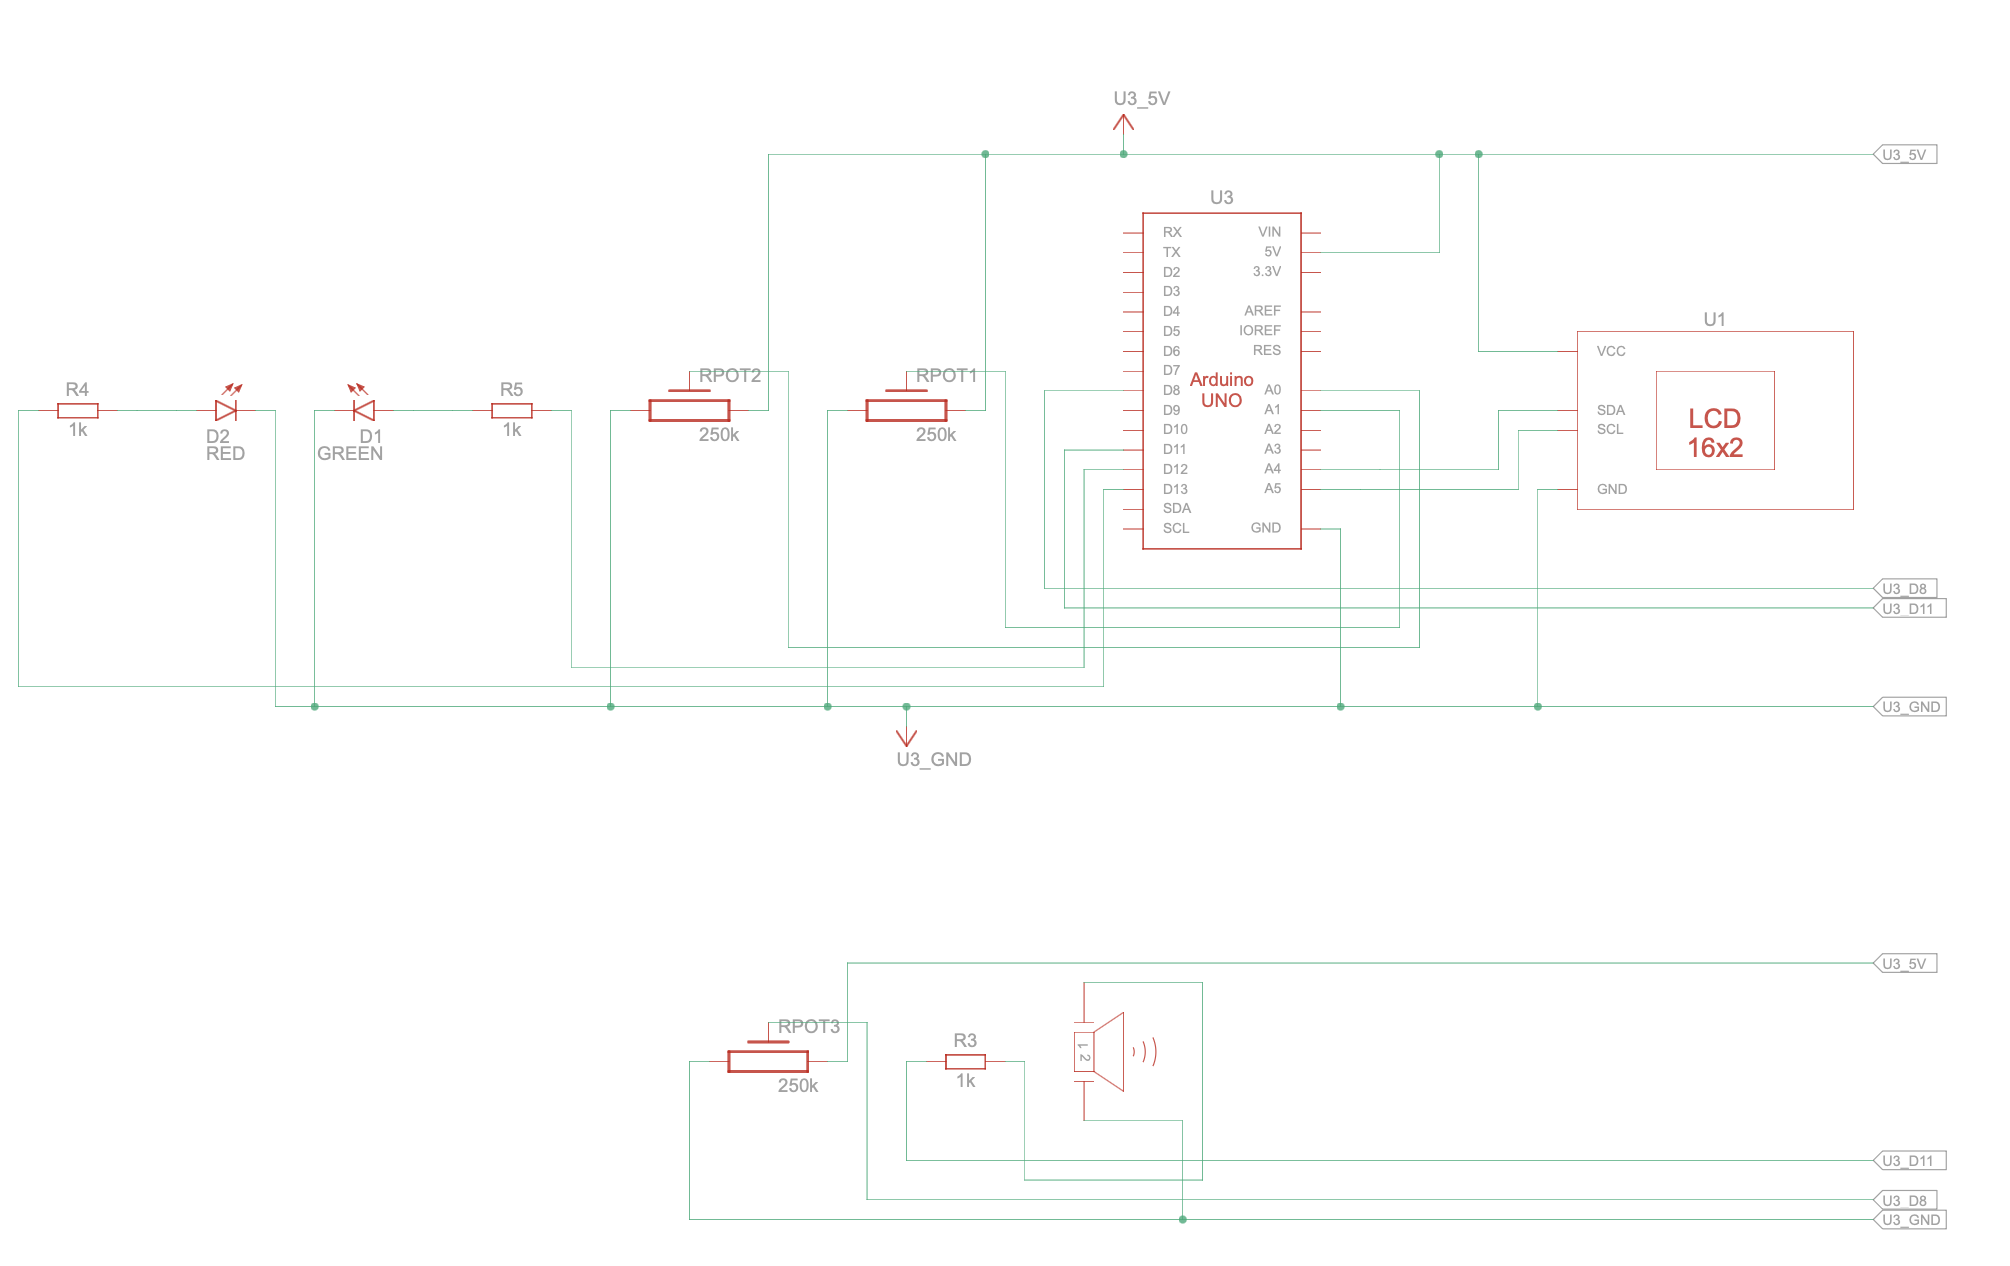
\includegraphics[width=0.92\textwidth]{electrical_schema.png}
\caption{Actual electrical schematic of the implemented circuit}
\label{fig:electrical-schema-real}
\end{figure}

\begin{figure}[H]
\centering
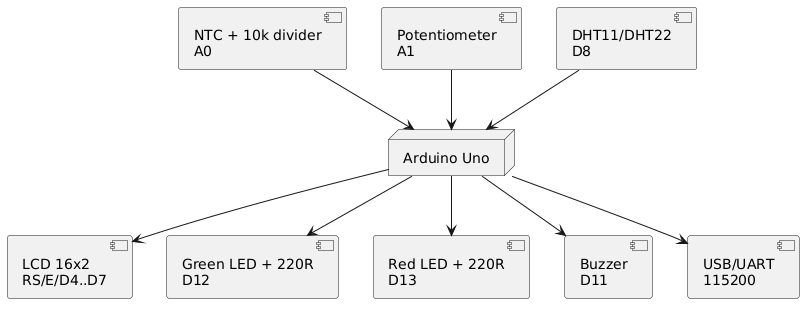
\includegraphics[width=0.88\textwidth]{electrical_block.png}
\caption{Functional electrical interconnection sketch -- Lab 5}
\label{fig:electrical-func}
\end{figure}

\textbf{Pin assignment:}
\begin{itemize}
    \item A0 -- NTC thermistor output (voltage divider, 10\,k$\Omega$ fixed to 5\,V)
    \item A1 -- Potentiometer output (dynamic setpoint input)
    \item D8 -- DHT22 data line (no external pull-up needed -- library uses internal)
    \item D2 -- LCD RS; D3 -- LCD Enable; D4--D7 -- LCD D4--D7 (4-bit mode)
    \item D12 -- Green LED + 220\,$\Omega$ resistor
    \item D13 -- Red LED + 220\,$\Omega$ resistor
    \item D11 -- Passive buzzer (PWM via \texttt{tone()})
    \item TX/D1 -- Serial UART to USB/PC at 115\,200 baud
\end{itemize}

\subsection{Project Directory Structure}

\begin{verbatim}
lab5/
|-- platformio.ini       <- env: uno (arduino, LiquidCrystal, DHT lib)
|-- diagram.json         <- Wokwi circuit definition
|-- wokwi.toml           <- Wokwi firmware pointer
|-- src/
|   |-- main.cpp         <- setup(): StdioBridge + app.begin(); loop(): app.tick()
|   |-- config/
|   |   `-- AppConfig.h  <- all pins, thresholds, timing, B-model constants
|   |-- sensors/
|   |   |-- NtcSensor.h/.cpp   <- ADC -> voltage -> resistance -> temperature
|   |   `-- DhtSensor.h/.cpp   <- DHT22 wrapper with NaN recovery
|   |-- signal/
|   |   `-- BinaryThresholdFilter.h/.cpp  <- hysteresis + persistence filter
|   |-- peripherals/
|   |   |-- LedController.h/.cpp   <- green/red LED pair
|   |   `-- BuzzerController.h/.cpp <- tone()/noTone() buzzer
|   |-- io/
|   |   |-- StdioBridge.h/.cpp   <- fdev_setup_stream -> Serial
|   |   `-- LcdDisplay.h/.cpp    <- LiquidCrystal 16x2 wrapper
|   `-- app/
|       `-- MonitorApp.h/.cpp    <- tick-based orchestration
`-- report/
    `-- main.tex
\end{verbatim}

Lab\,5 introduces a new \texttt{sensors/} layer (NTC + DHT22 drivers) and a \texttt{signal/} layer (\texttt{BinaryThresholdFilter}) not present in earlier labs, while removing the FreeRTOS dependency and task infrastructure.

\subsection{Software Module Descriptions}

\begin{itemize}
    \item \textbf{AppConfig.h}: Central configuration namespace. Pin assignments, timing periods, setpoint range (20--35\,°C), hysteresis half-band (1.0\,°C), B-model constants, serial baud rate.

    \item \textbf{NtcSensor}: Reads ADC raw via \texttt{analogRead()}, converts to voltage ($V = RAW \times V_{ref}/1023$), computes NTC resistance via voltage-divider inversion ($R_{NTC} = R_{fix} \cdot V / (V_{ref}-V)$), converts to temperature with the B-parameter equation ($1/T = 1/T_0 + \ln(R/R_0)/B$). Returns a \texttt{NtcSample} struct with all intermediate values for STDIO tracing.

    \item \textbf{DhtSensor}: Wraps the Adafruit DHT22 library. On each \texttt{readSample()} call, reads temperature; if \texttt{isnan(t)}, returns the last valid cached value with \texttt{fresh=false}. First read before any valid data returns \texttt{valid=false}.

    \item \textbf{BinaryThresholdFilter}: Implements hysteresis + persistence. \texttt{update(float valueC)} uses dynamic thresholds ($\geq T_{high}$ to enter, $\leq T_{low}$ to exit), while \texttt{setThresholds(high, low)} updates these thresholds at runtime from potentiometer input.

    \item \textbf{LedController}: ECAL wrapper exposing \texttt{setAlert(bool)}. \texttt{alert=true} turns green OFF and red ON; \texttt{alert=false} turns green ON and red OFF. Atomically updates both pins.

    \item \textbf{BuzzerController}: ECAL wrapper exposing \texttt{setAlert(bool)}. \texttt{alert=true} calls \texttt{tone(pin, 1000)}; \texttt{alert=false} calls \texttt{noTone(pin)}.

    \item \textbf{LcdDisplay}: Wraps \texttt{LiquidCrystal}. \texttt{showStatus()} formats fixed 16-character lines to avoid ghost symbols; row\,0 is ``N:xx.x D:xx.x'' (or ``n/a''), row\,1 shows ``TH:hh.h/ll.l'' and alert marker.

    \item \textbf{StdioBridge}: Registers \texttt{serial\_putchar} via \texttt{fdev\_setup\_stream} on \texttt{stdout} before the main loop starts. All \texttt{printf()} calls in any module automatically go to Serial UART.

    \item \textbf{MonitorApp}: Orchestrates all modules. Holds two \texttt{BinaryThresholdFilter} instances, latest \texttt{NtcSample}/\texttt{DhtSample}, potentiometer raw value, current setpoint, live thresholds and \texttt{\_systemAlert} flag. \texttt{tick(nowMs)} triggers acquisition at 40\,ms and reporting at 500\,ms.
\end{itemize}

\subsection{Reference to Source Code}

The full implementation is provided in the project repository linked in the annex. The report focuses on architecture, behaviour, testing, and validation evidence rather than inline code excerpts.

\subsection{Implementation Phase Conclusions}
\hspace{0.8cm} The implementation cleanly maps the design to code with no architectural surprises. Two important implementation notes:

\begin{enumerate}
    \item \textbf{Buzzer--DHT22 interference}: The DHT22 1-Wire protocol is timing-critical ($\leq$\,5\,$\mu$s bit timing). In Wokwi simulation, \texttt{tone()} uses a timer interrupt that can corrupt DHT22 bit sampling. The fix is to call \texttt{buzzer.setAlert(false)} immediately before each DHT22 read and restore the alert state after processing both sensors. This issue does not manifest on hardware (DHT22 uses external interrupts, not polling), but the defensive guard is kept for simulation correctness.
    \item \textbf{AVR \texttt{printf} and floats}: The default AVR \texttt{vfprintf} does not handle \texttt{\%f}/\texttt{\%e}/\texttt{\%g}. All floating-point values are pre-formatted via \texttt{dtostrf()} into local char buffers and printed with \texttt{\%s}. This avoids linking the heavy float printf variant ($\approx$\,2\,KB extra Flash).
\end{enumerate}

% ---------------------------------------------------------------------------
% SECTION 4 — TESTING AND VALIDATION
% ---------------------------------------------------------------------------
\section{Testing and Validation}

\subsection{Build Results}

\begin{table}[H]
\centering
\begin{tabular}{lrrrr}
\toprule
\textbf{Environment} & \textbf{Flash used} & \textbf{Flash \%} & \textbf{RAM used} & \textbf{RAM \%} \\
\midrule
\texttt{uno} & 14\,872 B & 46.1\% & 852 B & 41.6\% \\
\bottomrule
\end{tabular}
\caption{PlatformIO build resource usage (Lab 5)}
\label{tab:build}
\end{table}

The build completes with \texttt{[SUCCESS]}, zero errors, zero warnings. Flash and RAM usage remain within ATmega328P limits. The increased Flash relative to Lab\,4 reflects the Adafruit DHT library, LiquidCrystal library, and the NTC B-model floating-point math (requiring \texttt{log()} from AVR-libc).

\subsection{Test Execution Report}

\begin{longtable}{p{0.8cm} p{3.5cm} p{6.5cm} p{1.5cm}}
\toprule
\textbf{ID} & \textbf{Scenario} & \textbf{Observed result} & \textbf{Result} \\
\midrule
\endhead
T-01 & NTC cold (20°C) & Green LED ON; buzzer silent; STDIO stable=0 & PASS \\
T-02 & NTC hot ($\geq$27°C, 2 samples) & Red LED ON; buzzer 1kHz; STDIO stable=1 & PASS \\
T-03 & DHT cold (20°C) & No alert; Green LED & PASS \\
T-04 & DHT hot ($\geq$27°C, 2 samples) & Red LED + buzzer active; STDIO dht stable=1 & PASS \\
T-05 & Hysteresis around dynamic threshold & No alert state change; pendingCtr oscillates & PASS \\
T-06 & Single spike then back & pendingCtr reaches 1; stableHigh unchanged & PASS \\
T-07 & LCD row format & ``N: 24.3 D: 23.8'' / ``TH:28.1/26.1'' displayed & PASS \\
T-08 & STDIO report format & Full dump every 500ms with all fields present & PASS \\
T-09 & DHT NaN recovery & Cached temperature used; fresh=0 in STDIO & PASS \\
T-10 & Dual alert (both sensors high) & systemAlert=1; both sensor stableHigh=1 & PASS \\
T-11 & Alert latency & Alert activates within 80ms ($2\times40$ms) & PASS \\
T-12 & Memory check & Flash 46.1\%, RAM 41.6\% (both $<$ 100\%) & PASS \\
T-13 & Startup banner & Config banner printed once at init & PASS \\
T-14 & Potentiometer bonus & Setpoint and thresholds change while rotating potentiometer & PASS \\
\bottomrule
\caption{Test execution results -- Lab 5}
\label{tab:testresults}
\end{longtable}

All 14 test scenarios passed. The hysteresis and persistence tests (T-05, T-06) together with the potentiometer bonus test (T-14) confirm dynamic threshold operation and noise-resistant behavior.

\subsection{Simulation Screenshots}

\begin{figure}[H]
\centering
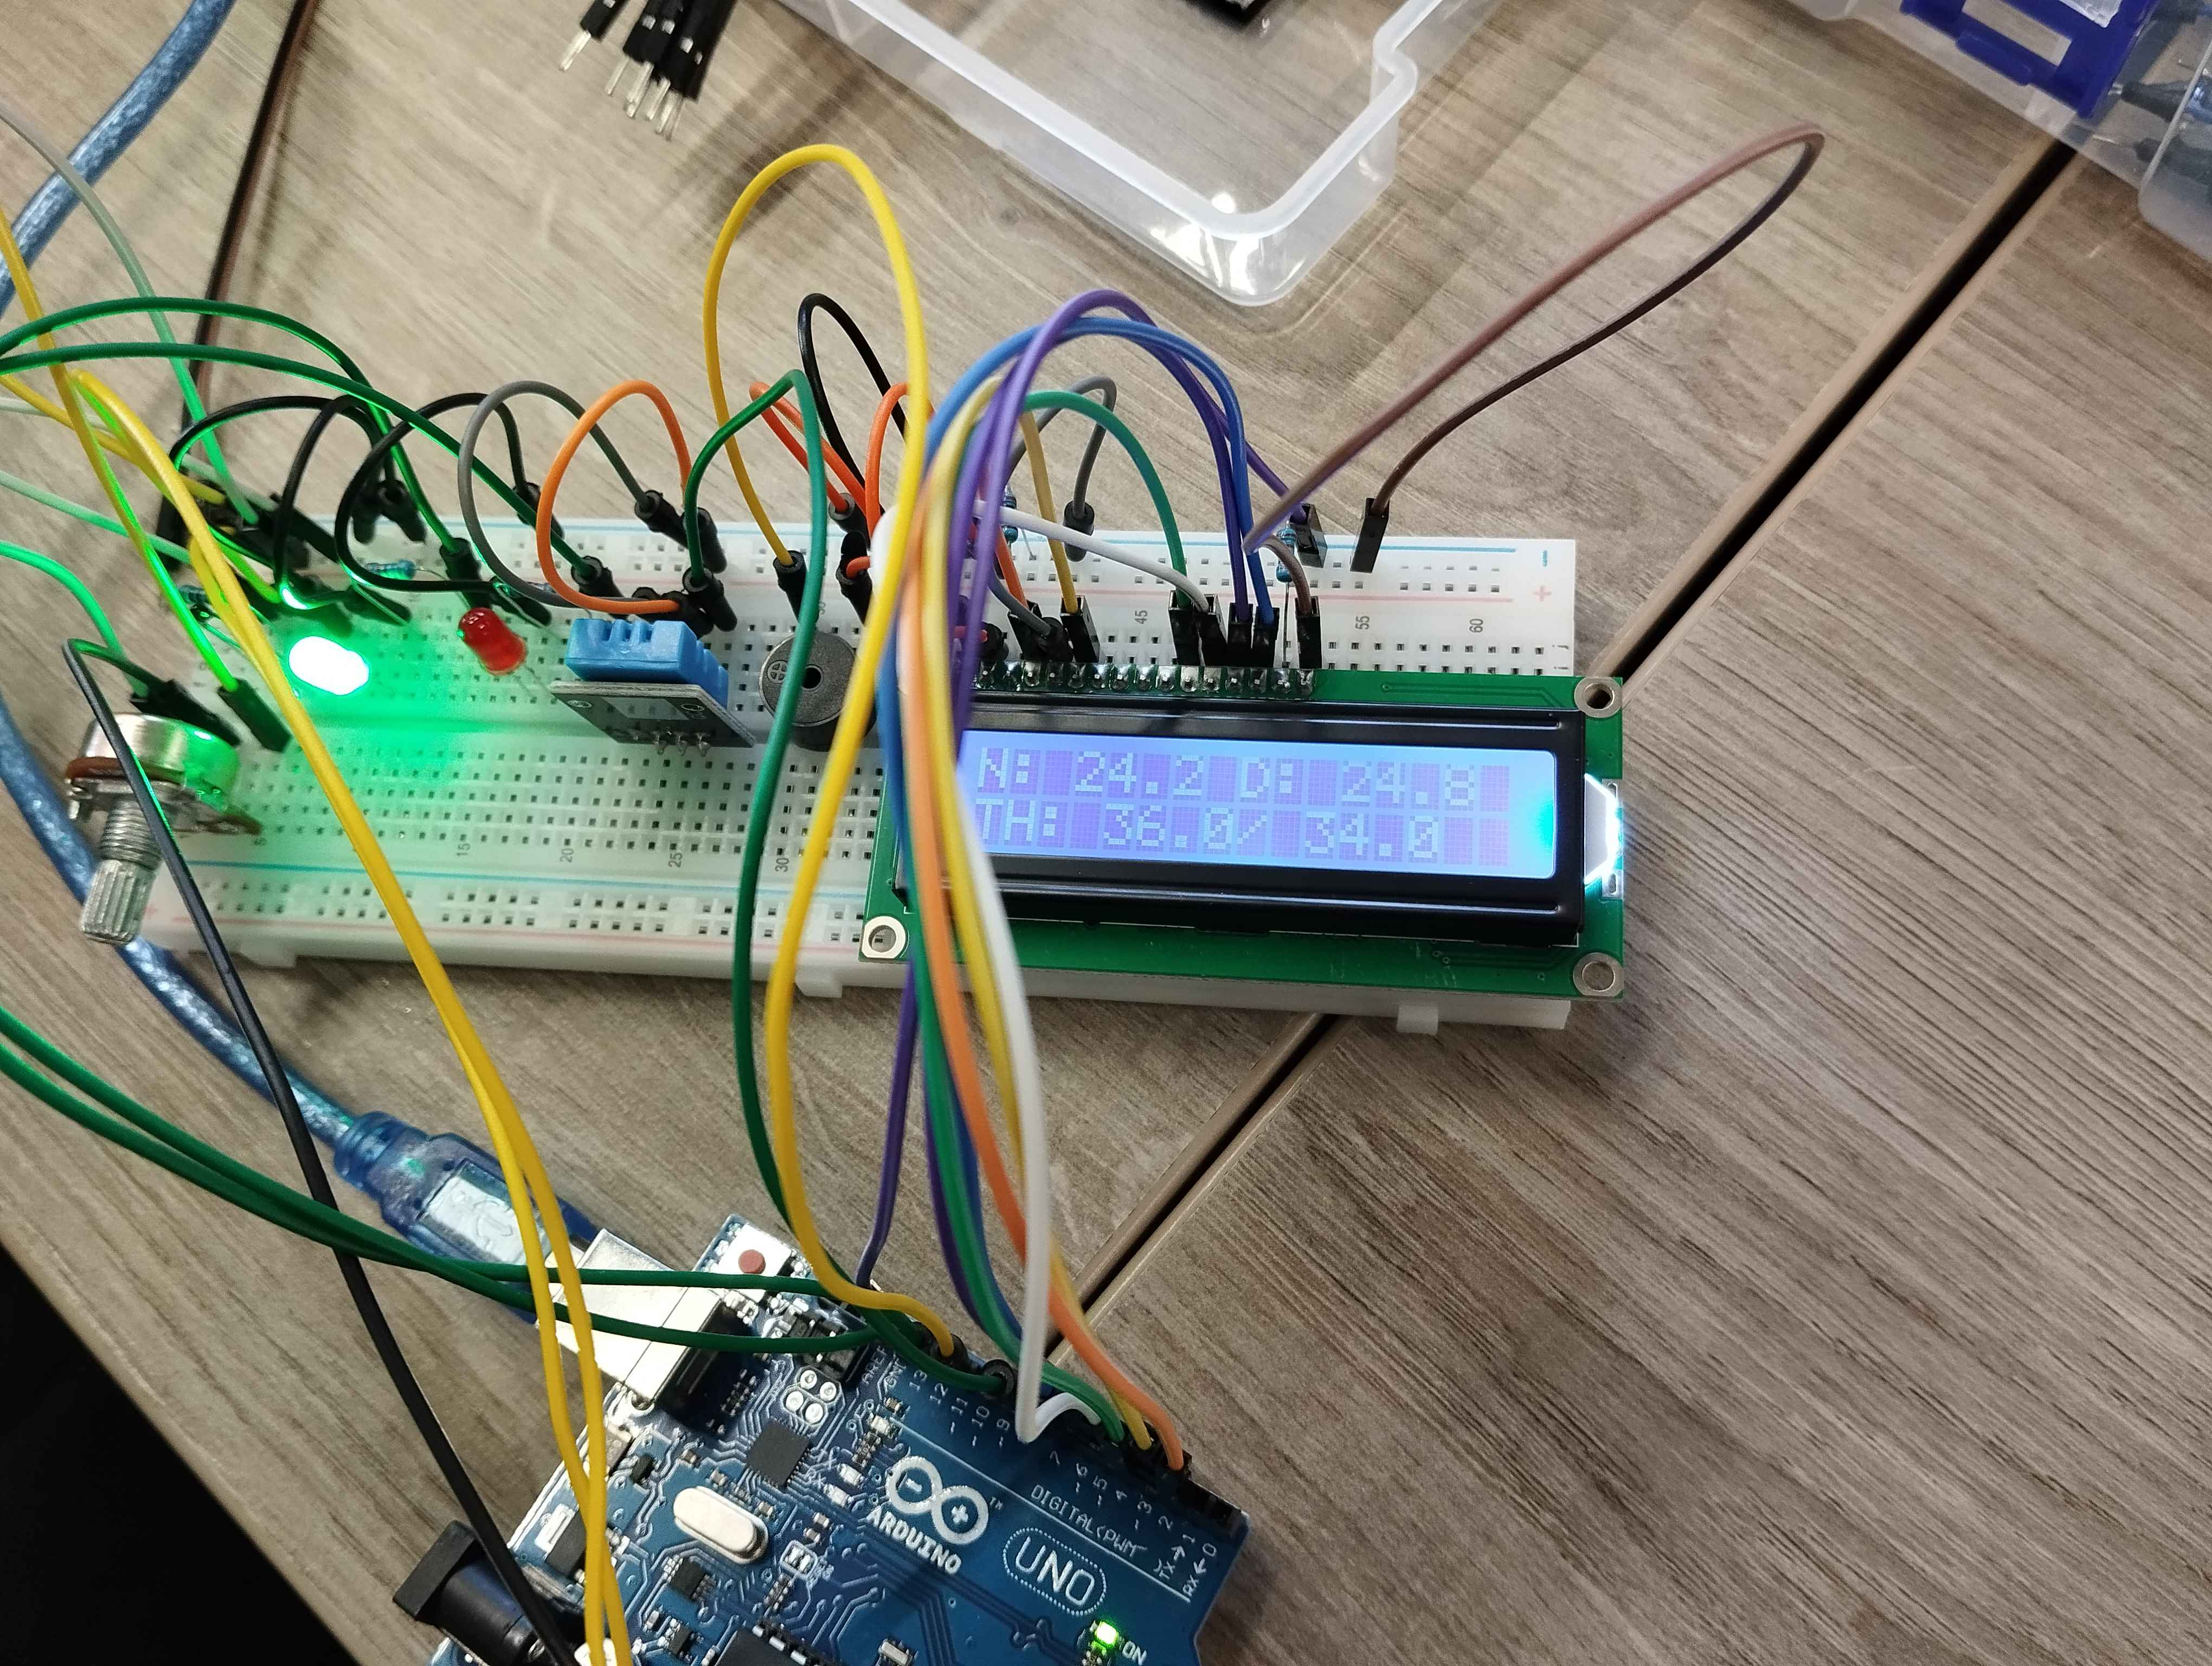
\includegraphics[width=0.8\textwidth]{hardware_no_alarm.jpg}
\caption{Wokwi simulation: normal operation -- Green LED, no alert on LCD}
\label{fig:wokwi-normal}
\end{figure}

\begin{figure}[H]
\centering
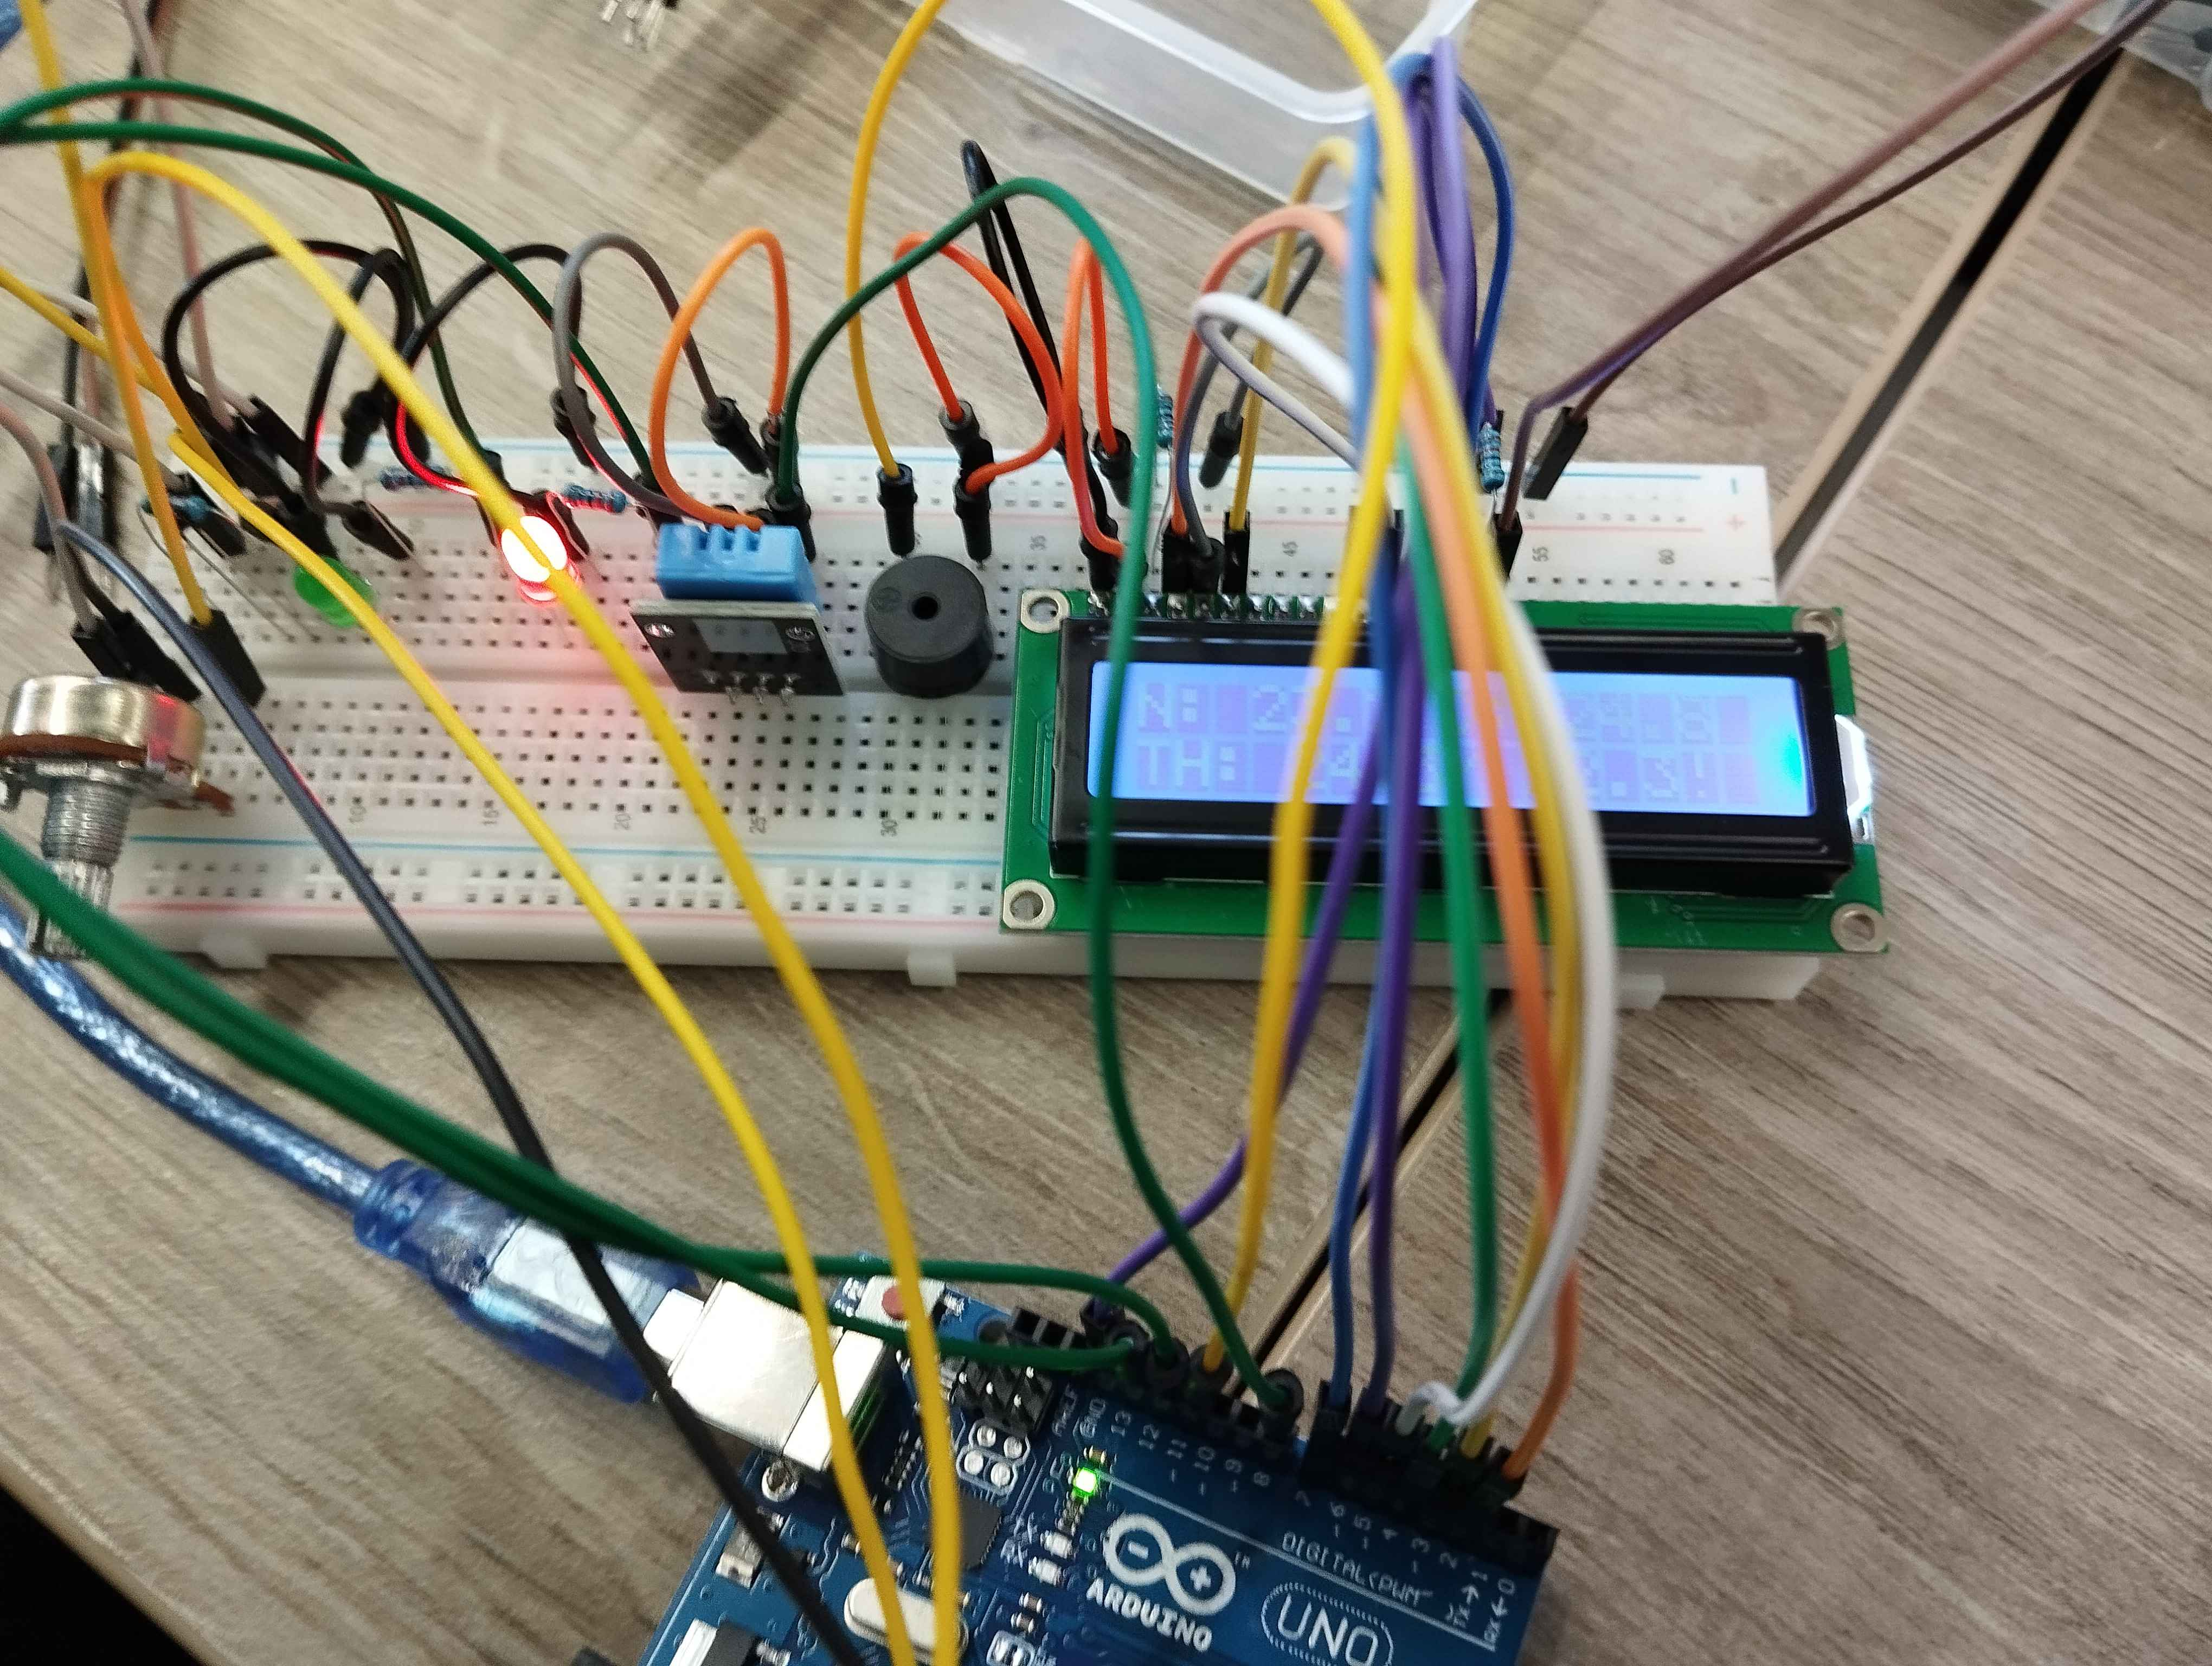
\includegraphics[width=0.8\textwidth]{hardware_alarm.jpg}
\caption{Wokwi simulation: alert state -- Red LED, buzzer, threshold row with alert marker}
\label{fig:wokwi-alert}
\end{figure}

\subsection{Representative Serial Output}

The following output was captured from a Wokwi simulation run with the NTC temperature raised to $\approx$\,27\,°C:

\begin{verbatim}
Lab5 - Dual sensor threshold monitor (NO FreeRTOS)
Sensors: NTC(A0 analog), DHT22(D8 digital)
Conditioning: hysteresis [dynamic], persistence=2 samples
Periods: acquisition=40ms, reporting=500ms, dht_min=2000ms
--------------------------------------------------------------
t=500ms
  NTC raw= 512 V= 2.50 T=  25.42C cand=0 stable=0 db=0
  DHT valid=1 fresh=1 T=  21.30C cand=0 stable=0 db=0
  SYS alert=0 LED_G=1 LED_R=0
    POT raw= 512 set=27.5C TH[ON>=28.5C OFF<=26.5C]
t=1000ms
  NTC raw= 447 V= 2.18 T=  27.14C cand=1 stable=0 db=1
  DHT valid=1 fresh=0 T=  21.30C cand=0 stable=0 db=0
  SYS alert=0 LED_G=1 LED_R=0
    POT raw= 530 set=27.8C TH[ON>=28.8C OFF<=26.8C]
t=1500ms
  NTC raw= 445 V= 2.17 T=  27.21C cand=1 stable=1 db=0
  DHT valid=1 fresh=0 T=  21.30C cand=0 stable=0 db=0
  SYS alert=1 LED_G=0 LED_R=1
    POT raw= 530 set=27.8C TH[ON>=28.8C OFF<=26.8C]
\end{verbatim}

The trace clearly shows the two-sample persistence: at \texttt{t=1000ms} the NTC candidate rises (\texttt{cand=1, db=1}) but the alert is not yet active. At \texttt{t=1500ms} the second confirming sample commits the transition (\texttt{stable=1, alert=1}).

\subsection{Performance Analysis}

\begin{itemize}
    \item \textbf{Alert latency}: Maximum time from threshold crossing to stable alert = 2 acquisition periods = 80\,ms. This satisfies R-NF-01 ($<$\,100\,ms).
    \item \textbf{CPU load}: The main loop \texttt{tick()} takes approximately 50--200\,$\mu$s per call (dominated by \texttt{log()} for NTC). With a 40\,ms acquisition period, CPU load is $<$\,0.5\% -- leaving ample margin for the serial ISR and LCD writes.
    \item \textbf{Float formatting}: \texttt{dtostrf()} each call requires $\approx$\,100\,$\mu$s and $\approx$\,50\,bytes of stack. Called 3 times per 500\,ms report cycle -- negligible.
    \item \textbf{DHT22 recharge window}: The Adafruit library internally enforces the 2\,s minimum read interval. The application's 40\,ms acquisition loop triggers \texttt{readSample()} every cycle; the library silently returns NaN (or cached data) for the 49 intermediate calls out of 50. The \texttt{fresh} flag in \texttt{DhtSample} distinguishes a new reading from a cached one.
    \item \textbf{Buzzer--DHT22 guard}: Silencing the buzzer for $<$\,10\,ms before the DHT22 read has no perceptible effect on the audible alert (the 40\,ms acquisition period is 4$\times$ longer than the gap). In hardware the guard is unnecessary but costs nothing.
\end{itemize}

\subsection{Testing Phase Conclusions}
\hspace{0.8cm} All 14 test scenarios passed. The most informative tests were T-05/T-06 (hysteresis and single-spike rejection) and T-14 (potentiometer bonus), which validate both filtering robustness and real-time threshold control. The STDIO trace format was designed specifically to make the pending counter and candidate/stable states visible for debugging.

% ---------------------------------------------------------------------------
% GENERAL CONCLUSIONS
% ---------------------------------------------------------------------------
\section*{General Conclusions}
\hspace{0.8cm} Laboratory Work \#5 achieved all stated objectives. A complete dual-sensor temperature monitoring application was designed, implemented, and validated on Arduino Uno, demonstrating the full signal conditioning chain from raw ADC/1-Wire data to a binary alert output with hysteresis and persistence filtering.

Key outcomes:
\begin{enumerate}
    \item \textbf{Multi-sensor acquisition}: Two fundamentally different sensor interfaces (analogue NTC thermistor via ADC, digital DHT22 via 1-Wire protocol) were integrated into a unified acquisition pipeline behind clean C++ interfaces (\texttt{NtcSensor}, \texttt{DhtSensor}).
    \item \textbf{B-parameter NTC model}: The Steinhart--Hart two-constant (B-parameter) equation converts NTC resistance to temperature accurately across the 0--50\,°C operating range, using only two calibration constants (\texttt{NtcBeta}, \texttt{NtcT0Kelvin}) stored in \texttt{AppConfig}.
    \item \textbf{Binary threshold conditioning}: The \texttt{BinaryThresholdFilter} demonstrates that reliable alert logic requires both hysteresis (a dead-band between the on/off thresholds) and persistence (N-sample confirmation) -- a single threshold is insufficient for noise immunity.
    \item \textbf{Cooperative multi-rate loop}: Decoupling the 40\,ms acquisition rate from the 500\,ms reporting rate, using independent \texttt{millis()} timestamps, is the simplest and most resource-efficient approach for multi-rate bare-metal embedded systems.
    \item \textbf{STDIO diagnostic reporting}: The \texttt{printf} report exposes all intermediate pipeline values (raw ADC, voltage, resistance, candidate/stable states, pending counter), turning the serial monitor into a full signal processing debugger without any additional tooling.
    \item \textbf{Modular architecture}: Six independent modules (\texttt{sensors}, \texttt{signal}, \texttt{peripherals}, \texttt{io}, \texttt{config}, \texttt{app}) communicate exclusively through struct interfaces, enabling independent unit testing and code reuse across laboratory projects.
\end{enumerate}

\textbf{Possible improvements:}
\begin{itemize}
    \item Add an exponential moving average (EMA) pre-filter before the threshold filter to reduce ADC quantisation noise on the NTC channel.
    \item Extend the report to include DHT22 humidity readings (the sensor provides them; only temperature is currently used).
    \item Port to FreeRTOS: a dedicated acquisition task (40\,ms periodic via \texttt{vTaskDelayUntil}) and a reporting task (500\,ms periodic) would further decouple the two activities and allow easy addition of more sensors.
    \item Use a FreeRTOS queue to pass \texttt{NtcSample}/\texttt{DhtSample} structs from the acquisition task to the reporting task, eliminating shared-variable access issues.
\end{itemize}

% ---------------------------------------------------------------------------
% UTM CRITERIA COVERAGE
% ---------------------------------------------------------------------------
\section*{Conformance with UTM Evaluation Criteria}
\begin{enumerate}
    \item \textbf{Technological analysis \& context}: Covered in Domain Analysis (technologies, HW/SW stack, application domain, design rationale).
    \item \textbf{Architectural design \& HW--SW explanations}: Covered via architecture section, interaction diagrams, and pin-level interconnection description.
    \item \textbf{Project structure \& modular implementation}: Covered in Project Directory Structure and Software Module Descriptions; separation of interfaces/implementations is preserved.
    \item \textbf{Hardware component description}: Each component (MCU, LEDs, resistors, LCD, DHT, NTC, potentiometer, breadboard) is documented with role.
    \item \textbf{Software module description}: Each module is listed and explained with its responsibilities and interactions.
    \item \textbf{Functional implementation}: Requirements and test tables demonstrate implementation completeness; behavioral diagrams are embedded as image evidence.
    \item \textbf{STDIO usage}: \texttt{printf} pipeline through \texttt{StdioBridge} is detailed; representative serial output is included.
    \item \textbf{Results presentation}: Diagram exports and simulation photos are included as visual evidence.
    \item \textbf{Report documentation}: Report includes analysis, design, implementation, testing, conclusions, bibliography ($\geq$3 references), AI usage note, and source-code annex.
    \item \textbf{Optional extra functionality}: Bonus feature implemented and documented: potentiometer-controlled dynamic setpoint/thresholds (A1).
\end{enumerate}

% ---------------------------------------------------------------------------
% AI TOOL USAGE
% ---------------------------------------------------------------------------
\section*{Note on AI Tool Usage}
\hspace{0.8cm} AI-assisted tools were used to support coding productivity and report drafting:
\begin{itemize}
    \item \textbf{GitHub Copilot} -- code suggestions, B-model implementation, DHT22 NaN recovery pattern.
    \item \textbf{LLM assistance} -- technical writing structure, LaTeX formatting, language polishing.
\end{itemize}
All generated content was manually reviewed, adapted, compiled, and validated against Wokwi simulation behaviour.

% ---------------------------------------------------------------------------
% BIBLIOGRAPHY
% ---------------------------------------------------------------------------
\section*{Bibliography}
\begin{enumerate}
    \item Horowitz, P., Hill, W. \textit{The Art of Electronics}, 3rd ed. Cambridge University Press, 2015.\\
    (NTC thermistor B-parameter model, voltage divider circuits.)

    \item Adafruit Industries. \textit{DHT22 / AM2302 Sensor Datasheet and Library}.\\
    \url{https://github.com/adafruit/DHT-sensor-library}

    \item Wokwi Simulator Documentation.\\
    \url{https://docs.wokwi.com/}

    \item PlatformIO Documentation -- library management, multi-dependency builds.\\
    \url{https://docs.platformio.org/en/latest/}

    \item AVR-libc Documentation -- \texttt{dtostrf}, \texttt{fdev\_setup\_stream}, ADC usage.\\
    \url{https://www.nongnu.org/avr-libc/user-manual/}

    \item Arduino Official Reference -- \texttt{analogRead}, \texttt{tone}, \texttt{LiquidCrystal}.\\
    \url{https://www.arduino.cc/reference/en/}

    \item Lab 5 Theory Notes -- Senzori: Achizitie si conditionare semnal.\\
    Technical University of Moldova, 2026.
\end{enumerate}

% ---------------------------------------------------------------------------
% ANNEX
% ---------------------------------------------------------------------------
\pagebreak
\section*{Annex -- Source Code}

The full source code is hosted on GitHub:

\bigskip
\noindent\textbf{Repository URL:}\\
\url{https://github.com/Ekkusuu/embedded-systems-repo/tree/main/lab5}

\bigskip
\noindent This repository contains all source files under \texttt{lab5/src/}, the PlatformIO configuration (\texttt{platformio.ini}), and the Wokwi simulation files (\texttt{diagram.json}, \texttt{wokwi.toml}).

\bigskip
\noindent PlantUML diagram source files used to generate the embedded diagram images are stored in:\\
\texttt{lab5/report/plantuml/}

\bigskip
\noindent\textbf{Complete module listing:}
\begin{itemize}
    \item \texttt{src/main.cpp} -- entry point, object instantiation, \texttt{setup()}/\texttt{loop()}
    \item \texttt{src/config/AppConfig.h} -- all compile-time constants
    \item \texttt{src/sensors/NtcSensor.h/.cpp} -- analogue NTC thermistor driver
    \item \texttt{src/sensors/DhtSensor.h/.cpp} -- DHT22 digital sensor wrapper
    \item \texttt{src/signal/BinaryThresholdFilter.h/.cpp} -- hysteresis + persistence filter
    \item \texttt{src/peripherals/LedController.h/.cpp} -- green/red LED pair driver
    \item \texttt{src/peripherals/BuzzerController.h/.cpp} -- passive buzzer driver
    \item \texttt{src/io/StdioBridge.h/.cpp} -- \texttt{fdev\_setup\_stream} UART bridge
    \item \texttt{src/io/LcdDisplay.h/.cpp} -- 16$\times$2 LCD wrapper
    \item \texttt{src/app/MonitorApp.h/.cpp} -- application orchestration
\end{itemize}

\end{document}
